\documentclass{article}

\usepackage{graphicx}
\usepackage{tikz}
\usepackage{tikzsymbols}
\usetikzlibrary{calc,patterns,shapes.geometric}
\pagestyle{empty}
\usepackage[margin=0pt]{geometry}
\geometry{papersize={14in,12in}}

\def\centerarc[#1](#2)(#3:#4:#5){\draw[#1] ($(#2)+({#5*cos(#3)},{#5*sin(#3)})$) arc (#3:#4:#5);}

\begin{document}
	\begin{figure}
		\centering
		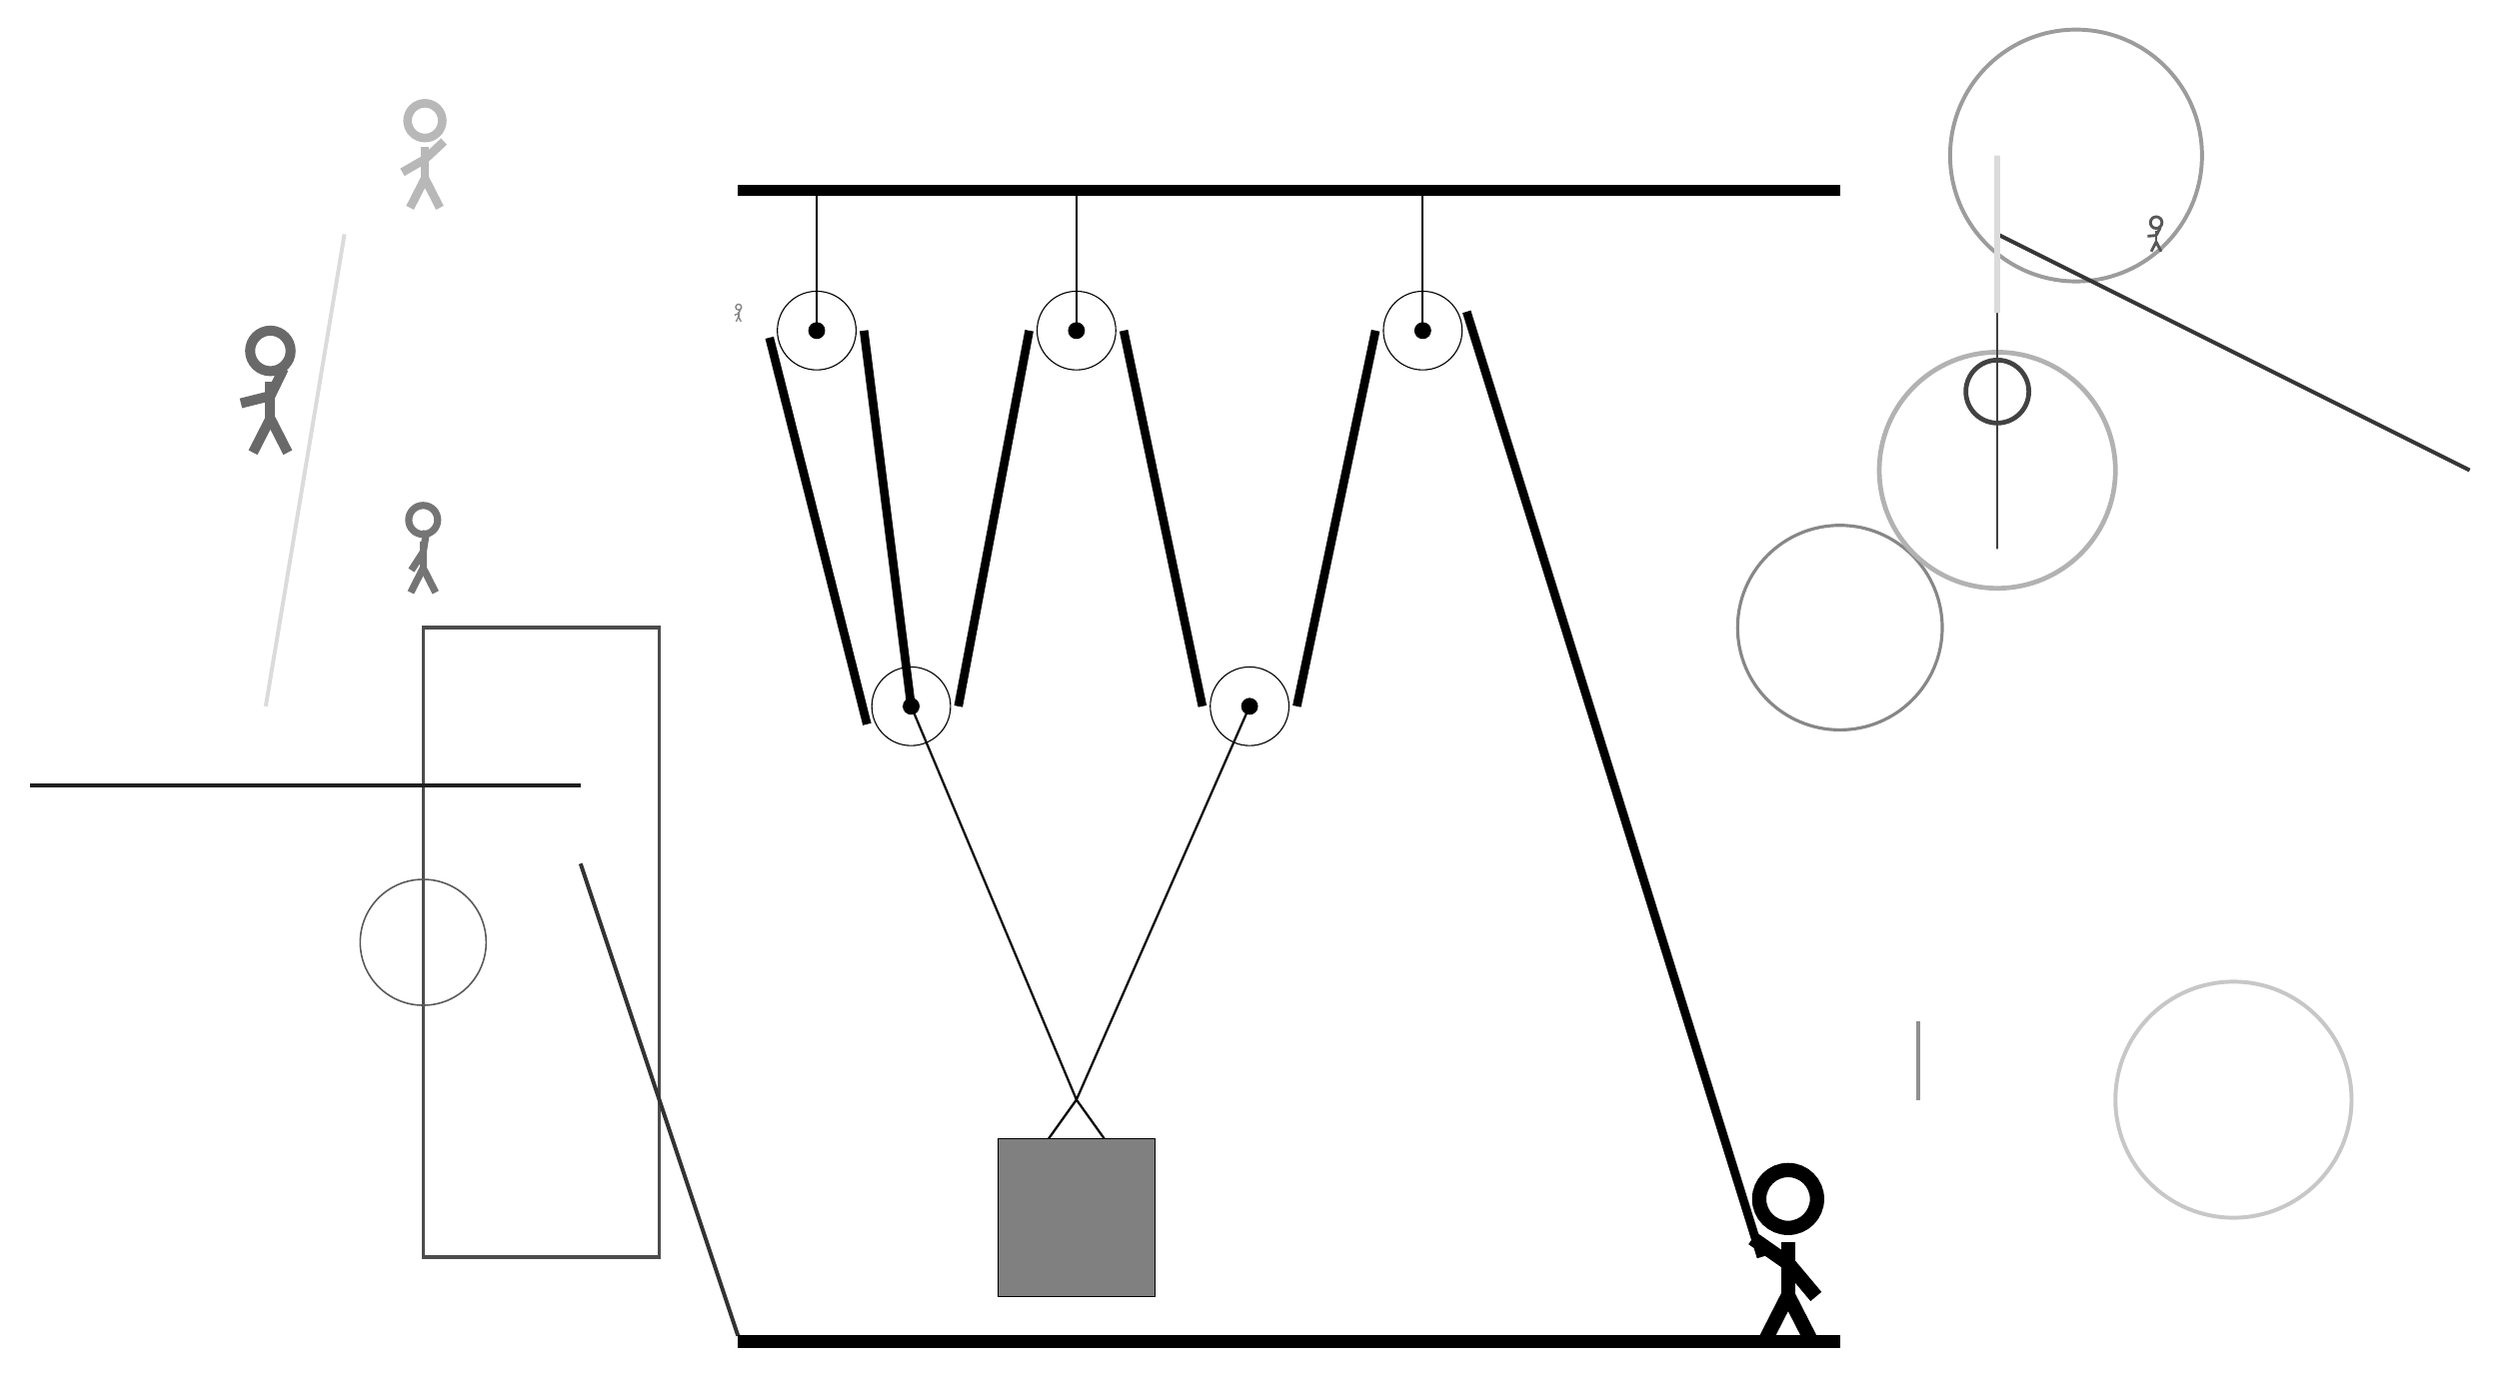
\begin{tikzpicture}
			%%%%% START %%%%%
			
			\draw[fill=black] (-2, 11.5) rectangle (12, 11.625);
			
			\draw (-1, 9.775) circle (0.5);
			\draw[fill=black] (-1, 9.775) circle (0.1);
			\draw[thick] (-1, 9.775) -- (-1, 11.5);
			
			\draw [line width=0.5mm, color=black!39](15, 12) circle (1.6);
			
			\draw [line width=0.5mm, color=black!22](17, 0) circle (1.5);
			\draw [line width=0.4mm, color=black!47](12, 6) circle (1.3);
			\draw[line width=0.4mm, color=black!70] (-3, 6) rectangle (-6, -2);
			
			\node[line width=0.2mm, color=black!28] at (-6, 12) {\Strichmaxerl[6][30][43]};
			
			\draw[line width=0.5mm, color=black!88](-4, 4) -- (-11, 4);
			\node[line width=0.4mm, color=black!54] at (-6, 7) {\Strichmaxerl[5][57][81]};
			\node[line width=0.2mm, color=black!47] at (-2, 10) {\Strichmaxerl[1][22][66]};
			\node[line width=0.3mm, color=black!66] at (16, 11) {\Strichmaxerl[2][5][62]};
			\draw [line width=0.6mm, color=black!30](14, 8) circle (1.5);
			\draw[line width=0.5mm, color=black!79](14, 11) -- (20, 8);
			\draw[line width=0.3mm, color=black!75] (14, 7) rectangle (14, 11);
			\draw[line width=0.5mm, color=black!80](-2, -3) -- (-4, 3);
			\draw [line width=0.6mm, color=black!74](14, 9) circle (0.4);
			\node[line width=0.3mm, color=black!59] at (-8, 9) {\Strichmaxerl[7][14][64]};
			\draw[line width=0.2mm, color=black!77] (-2, 6) rectangle (-2, 6);
			
			\draw[line width=0.5mm, color=black!14](-7, 11) -- (-8, 5);
			\draw[line width=0.5mm, color=black!44](13, 1) -- (13, 0);
			\draw[line width=0.7mm, color=black!14] (14, 10) rectangle (14, 12);
			
			\draw [line width=0.2mm, color=black!65](-6, 2) circle (0.8);
			
			\draw (2.3, 9.775) circle (0.5);
			\draw[fill=black] (2.3, 9.775) circle (0.1);
			\draw[thick] (2.3, 9.775) -- (2.3, 11.5);
			
			\draw (6.7, 9.775) circle (0.5);
			\draw[fill=black] (6.7, 9.775) circle (0.1);
			\draw[thick] (6.7, 9.775) -- (6.7, 11.5);
			
			\draw (0.2, 5) circle (0.5);
			\draw[fill=black] (0.2, 5) circle (0.1);
			
			\draw (4.5, 5) circle (0.5);
			\draw[fill=black] (4.5, 5) circle (0.1);
			
			\draw[thick] (0.2, 5) -- (2.3, 0)  -- (4.5, 5);
			\draw[thick]  (1.8, -0.7) -- (2.3, 0) -- (2.8, -0.7);
			\draw[fill=black!50] (1.3, -0.5) rectangle (3.3, -2.5);
			
			\draw[line width=1.1mm] (0.2, 5) -- (-0.4, 9.775);
			\centerarc[line width=1.1mm](-1, 9.775)(0:200:0.6);
			\draw[line width=1.1mm] (-1.6, 9.685) -- (-0.361, 4.772);
			\centerarc[line width=1.1mm](0.2, 5)(200:360:0.6);
			\draw[line width=1.1mm](0.8, 5) -- (1.7, 9.775);
			\centerarc[line width=1.1mm](2.3, 9.775)(0:180:0.6);
			\draw[line width=1.1mm] (2.9, 9.775) -- (3.9, 5);
			\centerarc[line width=1.1mm](4.5, 5)(180:360:0.6);
			\draw[line width=1.1mm] (5.1, 5) -- (6.1, 9.775);
			\centerarc[line width=1.1mm](6.7, 9.775)(20:180:0.6);
			\draw[line width=1.1mm](7.258, 10.015)  -- (11, -2);
			
			\node at (11.3, -2) {\Strichmaxerl[10][-35][-50]};
			
			\draw[fill=black] (-2, -3) rectangle (12, -3.15);
			
			%%%%% END %%%%%
		\end{tikzpicture}
	\end{figure}	
\end{document}